%!TEX root = report.tex
Running the Min-Over algorithm on a student perceptron yields a few interesting results. 

The generalization error determines the probability that disagreement occurs between the teacher perceptron and the student perceptron. Figure~\ref{fig:generalizationerror} plots the generalization error as a function of the time.
\myfigure{
	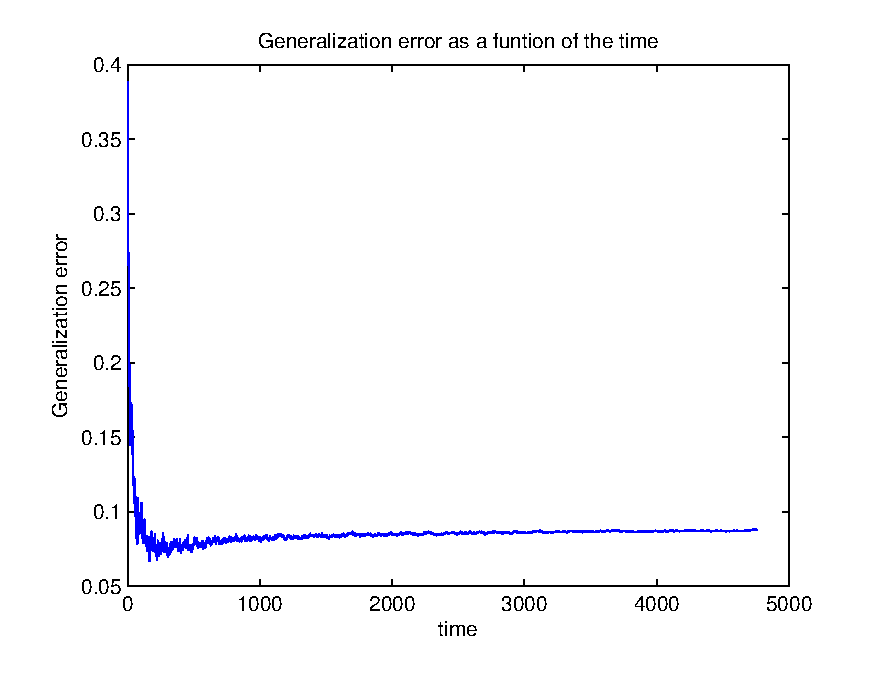
\includegraphics[width=\columnwidth]{generalizationerror.eps}%
	\figcaption{The generalization error as a function of the time. Note it converges quite fast.}
	\label{fig:generalizationerror}
}

It can be seen in figure~\ref{fig:generalizationerror} that error converges relatively fast towards a certain value. We have found that for noise-free learning the value it converges towards is around  $\frac{1}{10}$.